\documentclass[tikz,border=8pt]{standalone}
% Estilos del modelo C4 para TikZ (colores y formas de C4). Los tres diagramas del informe los cargan con \input.
\usepackage{fontspec}
\usepackage{xcolor}
\usetikzlibrary{shapes.geometric,arrows.meta,positioning,calc,fit,backgrounds}
\renewcommand{\familydefault}{\sfdefault}
\hyphenpenalty=10000 \exhyphenpenalty=10000 % sin guiones al partir las palabras en las cajas

\definecolor{c4persona}{HTML}{08427B}   \definecolor{c4personab}{HTML}{073B6F}
\definecolor{c4sistema}{HTML}{1168BD}   \definecolor{c4sistemab}{HTML}{0B4884}
\definecolor{c4externo}{HTML}{999999}   \definecolor{c4externob}{HTML}{6B6B6B}
\definecolor{c4cont}{HTML}{438DD5}      \definecolor{c4contb}{HTML}{3C7FC0}
\definecolor{c4comp}{HTML}{85BBF0}      \definecolor{c4compb}{HTML}{78A8D8}

% \elem{Nombre}{[Tipo: tecnología]}{Descripción}: el texto de un elemento en tres líneas, como en C4.
\newcommand{\elem}[3]{\textbf{#1}\\[1pt]{\scriptsize #2}\if\relax\detokenize{#3}\relax\else\\[3pt]{\scriptsize #3}\fi}

\tikzset{
  c4box/.style={draw, rounded corners=4pt, align=center, inner sep=5pt, text=white, font=\sffamily\small,
                text width=3.1cm, minimum height=2.0cm},
  persona/.style={c4box, fill=c4persona, draw=c4personab},
  sistema/.style={c4box, fill=c4sistema, draw=c4sistemab},
  externo/.style={c4box, fill=c4externo, draw=c4externob},
  contenedor/.style={c4box, fill=c4cont, draw=c4contb},
  componente/.style={c4box, fill=c4comp, draw=c4compb, text=black},
  basedatos/.style={contenedor, shape=cylinder, shape border rotate=90, aspect=0.16, minimum height=2.4cm},
  limite/.style={draw=c4externob, dashed, rounded corners=6pt, inner sep=0.45cm},
  rel/.style={-{Stealth[length=2.4mm,width=1.9mm]}, line width=0.7pt, color=black!70},
  etq/.style={fill=white, inner sep=1.5pt, align=center, font=\sffamily\scriptsize, text=black!85},
}

% Cabeza de una persona (se dibuja detrás de su caja): \cabeza{nombre de la caja}
\newcommand{\cabeza}[1]{\begin{scope}[on background layer]\node[circle, fill=c4persona, draw=c4personab, minimum size=0.9cm] at ([yshift=0.18cm]#1.north) {};\end{scope}}

\begin{document}
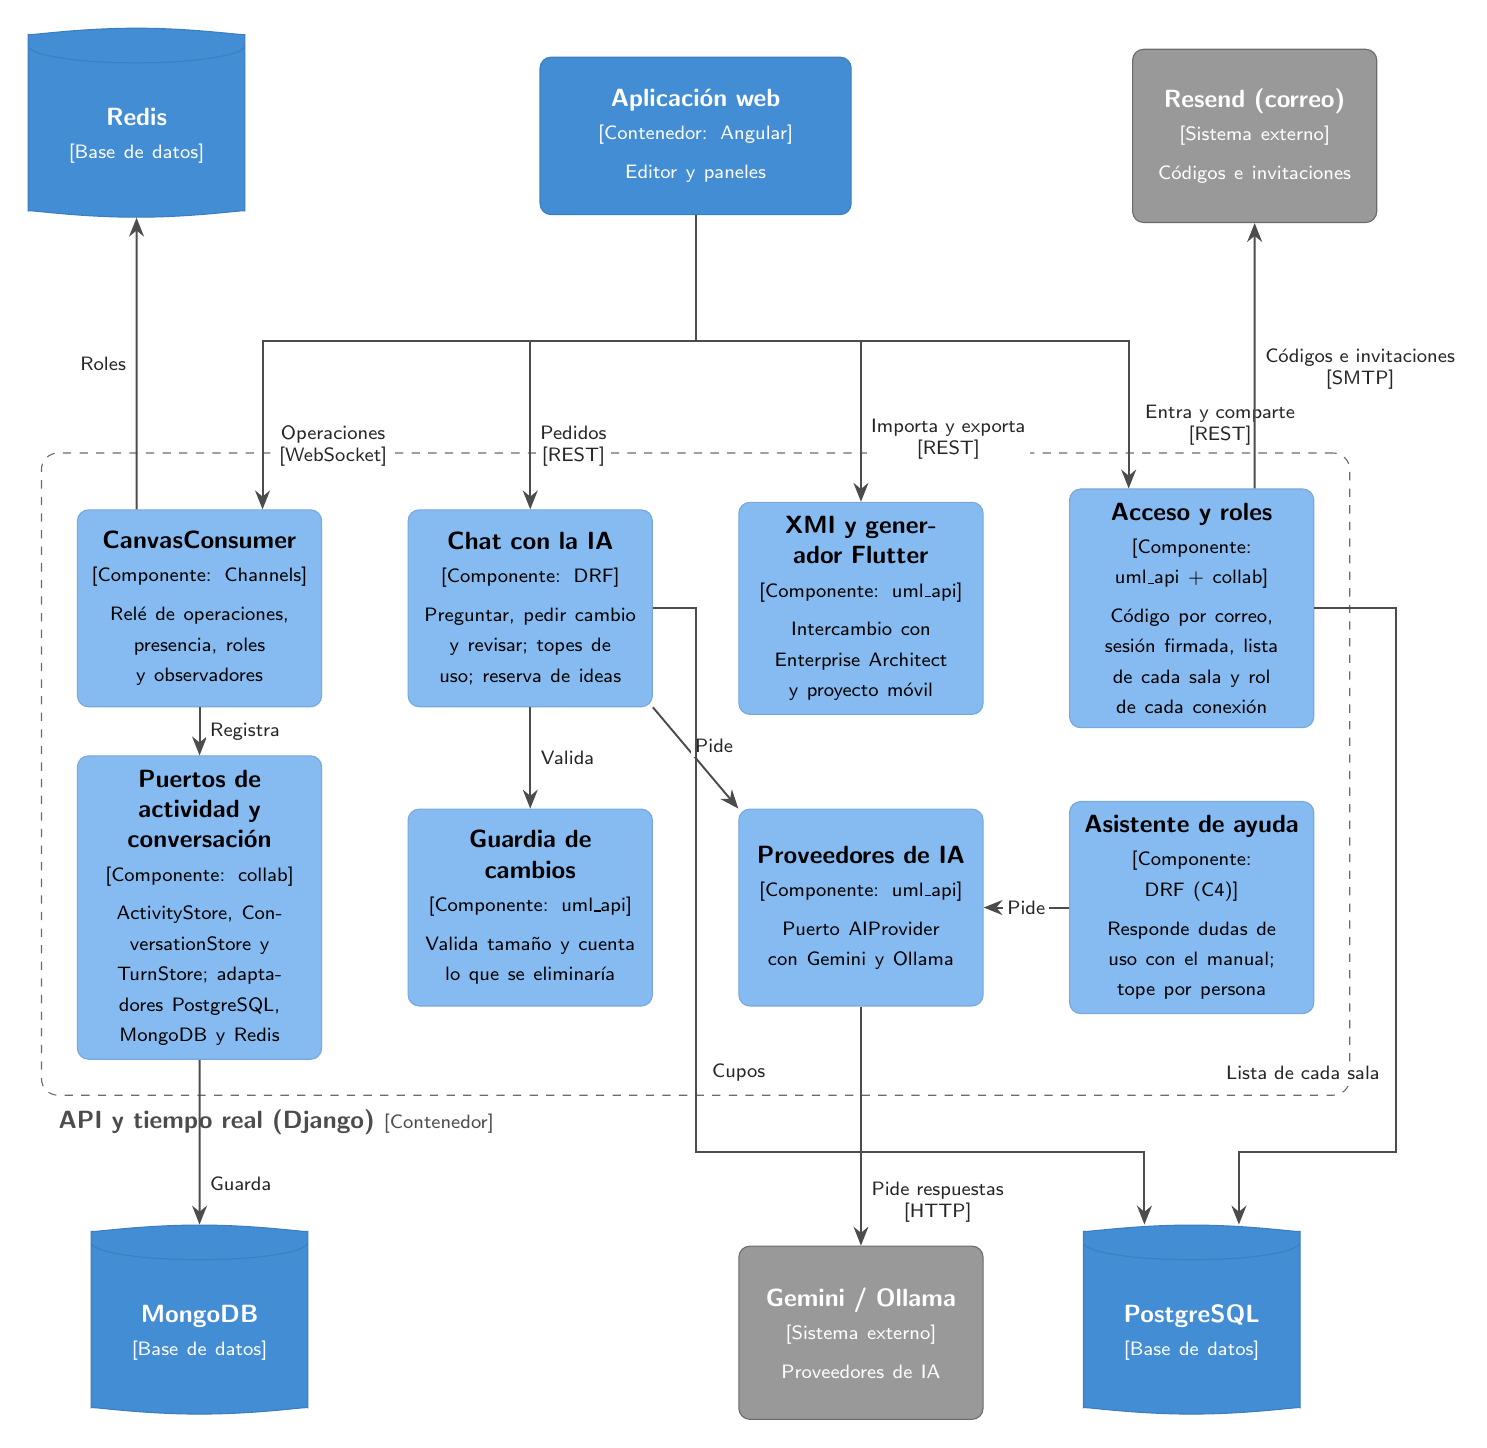
\begin{tikzpicture}
  % 4 columnas a 4.2 cm. Fila de arriba (A): los componentes que llama la aplicación web; fila del medio (B): el resto. Fuera del límite: arriba
  % Redis y el correo, abajo MongoDB, los proveedores de IA y PostgreSQL.
  \tikzset{comp/.style={componente, text width=2.75cm, minimum height=2.5cm}}
  \node[contenedor, text width=3.6cm, minimum height=2.0cm] (web) at (6.3, 6.0) {\elem{Aplicación web}{[Contenedor: Angular]}{Editor y paneles}};

  \node[comp] (canvas) at (0, 0) {\elem{CanvasConsumer}{[Componente: Channels]}{Relé de operaciones, presencia, roles y observadores}};
  \node[comp] (chat)   at (4.2, 0) {\elem{Chat con la IA}{[Componente: DRF]}{Preguntar, pedir cambio y revisar; topes de uso; reserva de ideas}};
  \node[comp] (xmi)    at (8.4, 0) {\elem{XMI y generador Flutter}{[Componente: uml\_api]}{Intercambio con Enterprise Architect y proyecto móvil}};
  \node[comp] (acceso) at (12.6, 0) {\elem{Acceso y roles}{[Componente: uml\_api + collab]}{Código por correo, sesión firmada, lista de cada sala y rol de cada conexión}};
  \node[comp] (stores) at (0,-3.8) {\elem{Puertos de actividad y conversación}{[Componente: collab]}{ActivityStore, ConversationStore y TurnStore; adaptadores PostgreSQL, MongoDB y Redis}};
  \node[comp] (guard)  at (4.2,-3.8) {\elem{Guardia de cambios}{[Componente: uml\_api]}{Valida tamaño y cuenta lo que se eliminaría}};
  \node[comp] (provider) at (8.4,-3.8) {\elem{Proveedores de IA}{[Componente: uml\_api]}{Puerto AIProvider con Gemini y Ollama}};
  \node[comp] (ayuda)  at (12.6,-3.8) {\elem{Asistente de ayuda}{[Componente: DRF (C4)]}{Responde dudas de uso con el manual; tope por persona}};

  \begin{scope}[on background layer]
    \node[limite, fit=(canvas)(chat)(xmi)(acceso)(stores)(guard)(provider)(ayuda)] (lim) {};
  \end{scope}
  \node[anchor=north west, font=\sffamily\small\bfseries, text=black!70] at ([xshift=0.1cm,yshift=-0.05cm]lim.south west) {API y tiempo real (Django) \normalfont\scriptsize [Contenedor]};

  \node[basedatos, text width=2.4cm, minimum height=2.4cm] (rd) at (-0.8, 6.0) {\elem{Redis}{[Base de datos]}{}};
  \node[externo, text width=2.75cm, minimum height=2.2cm] (correo) at (13.4, 6.0) {\elem{Resend (correo)}{[Sistema externo]}{Códigos e invitaciones}};
  \node[basedatos, text width=2.4cm, minimum height=2.4cm] (mg) at (0,-9.2) {\elem{MongoDB}{[Base de datos]}{}};
  \node[externo, text width=2.75cm, minimum height=2.2cm] (prov) at (8.4,-9.2) {\elem{Gemini / Ollama}{[Sistema externo]}{Proveedores de IA}};
  \node[basedatos, text width=2.4cm, minimum height=2.4cm] (pg) at (12.6,-9.2) {\elem{PostgreSQL}{[Base de datos]}{}};

  % la aplicación web llama a cuatro componentes
  \coordinate (bus) at (0, 3.4);
  \draw[rel] (web.south) -- (web.south |- bus) -| ([xshift=0.8cm]canvas.north);
  \draw[rel] (web.south) -- (web.south |- bus) -| (chat.north);
  \draw[rel] (web.south) -- (web.south |- bus) -| (xmi.north);
  \draw[rel] (web.south) -- (web.south |- bus) -| ([xshift=-0.8cm]acceso.north);
  \node[etq, anchor=west] at ([xshift=0.95cm,yshift=0.8cm]canvas.north) {Operaciones\\{[WebSocket]}};
  \node[etq, anchor=west] at ([xshift=2pt,yshift=0.8cm]chat.north) {Pedidos\\{[REST]}};
  \node[etq, anchor=west] at ([xshift=2pt,yshift=0.8cm]xmi.north) {Importa y exporta\\{[REST]}};
  \node[etq, anchor=west] at ([xshift=-0.65cm,yshift=0.8cm]acceso.north) {Entra y comparte\\{[REST]}};

  % Redis y el correo, en vertical sobre su componente
  \draw[rel] ([xshift=-0.8cm]canvas.north) -- node[etq, anchor=east, xshift=-2pt] {Roles} (rd.south);
  \draw[rel] ([xshift=0.8cm]acceso.north) -- node[etq, anchor=west, xshift=2pt, pos=0.45] {Códigos e invitaciones\\{[SMTP]}} (correo.south);

  \draw[rel] (canvas) -- node[etq, anchor=west, xshift=2pt] {Registra} (stores);
  \draw[rel] (chat) -- node[etq, anchor=west, xshift=2pt] {Valida} (guard);
  \draw[rel] (chat.south east) -- node[etq, pos=0.5, anchor=south west, xshift=-2pt] {Pide} (provider.north west);
  \draw[rel] (ayuda) -- node[etq] {Pide} (provider);
  \draw[rel] (stores) -- node[etq, anchor=west, xshift=2pt, pos=0.75] {Guarda} (mg);
  \draw[rel] (provider) -- node[etq, anchor=west, xshift=2pt, pos=0.82] {Pide respuestas\\{[HTTP]}} (prov);

  % cupos de uso (chat) y lista de cada sala (acceso) llegan a PostgreSQL
  \draw[rel] (chat.east) -- (6.3, 0) -- (6.3,-6.9) -- ([xshift=-0.6cm]pg.north |- 0,-6.9) -- ([xshift=-0.6cm]pg.north);
  \draw[rel] (acceso.east) -- (15.2, 0) -- (15.2,-6.9) -- ([xshift=0.6cm]pg.north |- 0,-6.9) -- ([xshift=0.6cm]pg.north);
  \node[etq, anchor=west] at (6.45,-5.9) {Cupos};
  \node[etq, anchor=east] at (15.05,-5.9) {Lista de cada sala};
\end{tikzpicture}
\end{document}
